\section{State of 14e/19o plots}
\begin{frame}
\frametitle{State of 14e/19o plots}
\begin{figure}
    \centering
    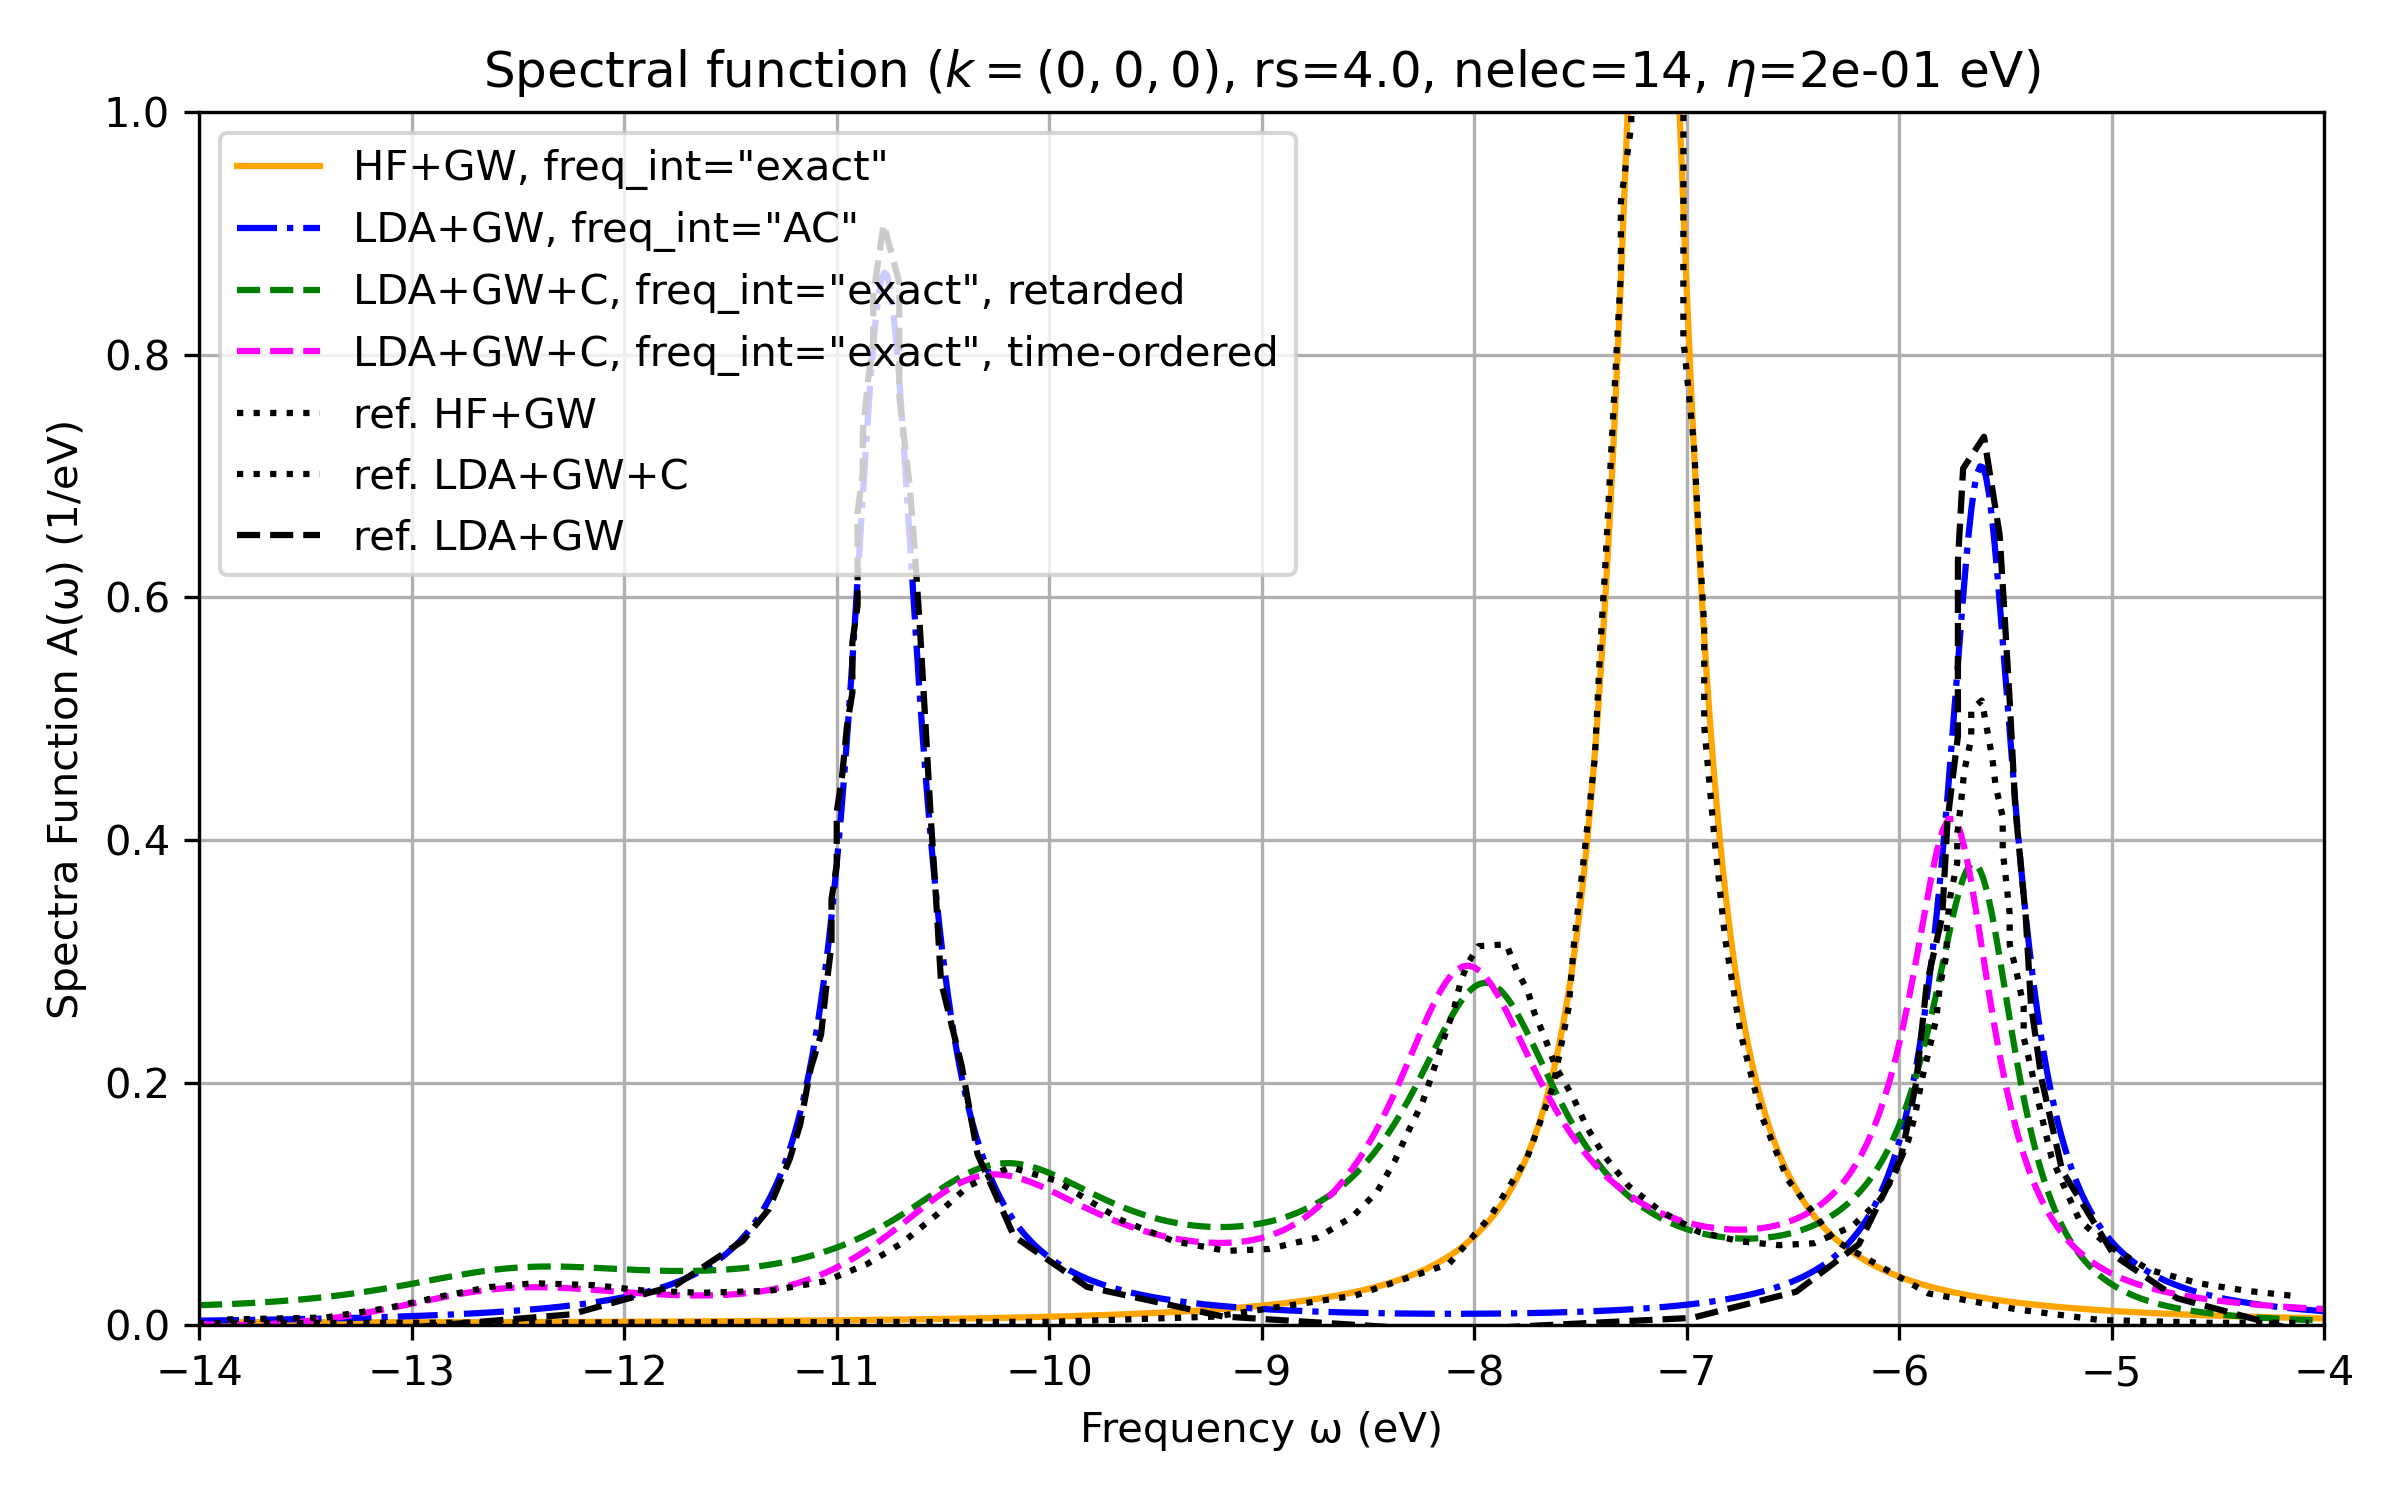
\includegraphics[width=\textwidth]{figs/image.png}
\end{figure}
\end{frame}
\begin{frame}
\frametitle{State of 14e/19o plots cont.}
\begin{figure}
    \centering
    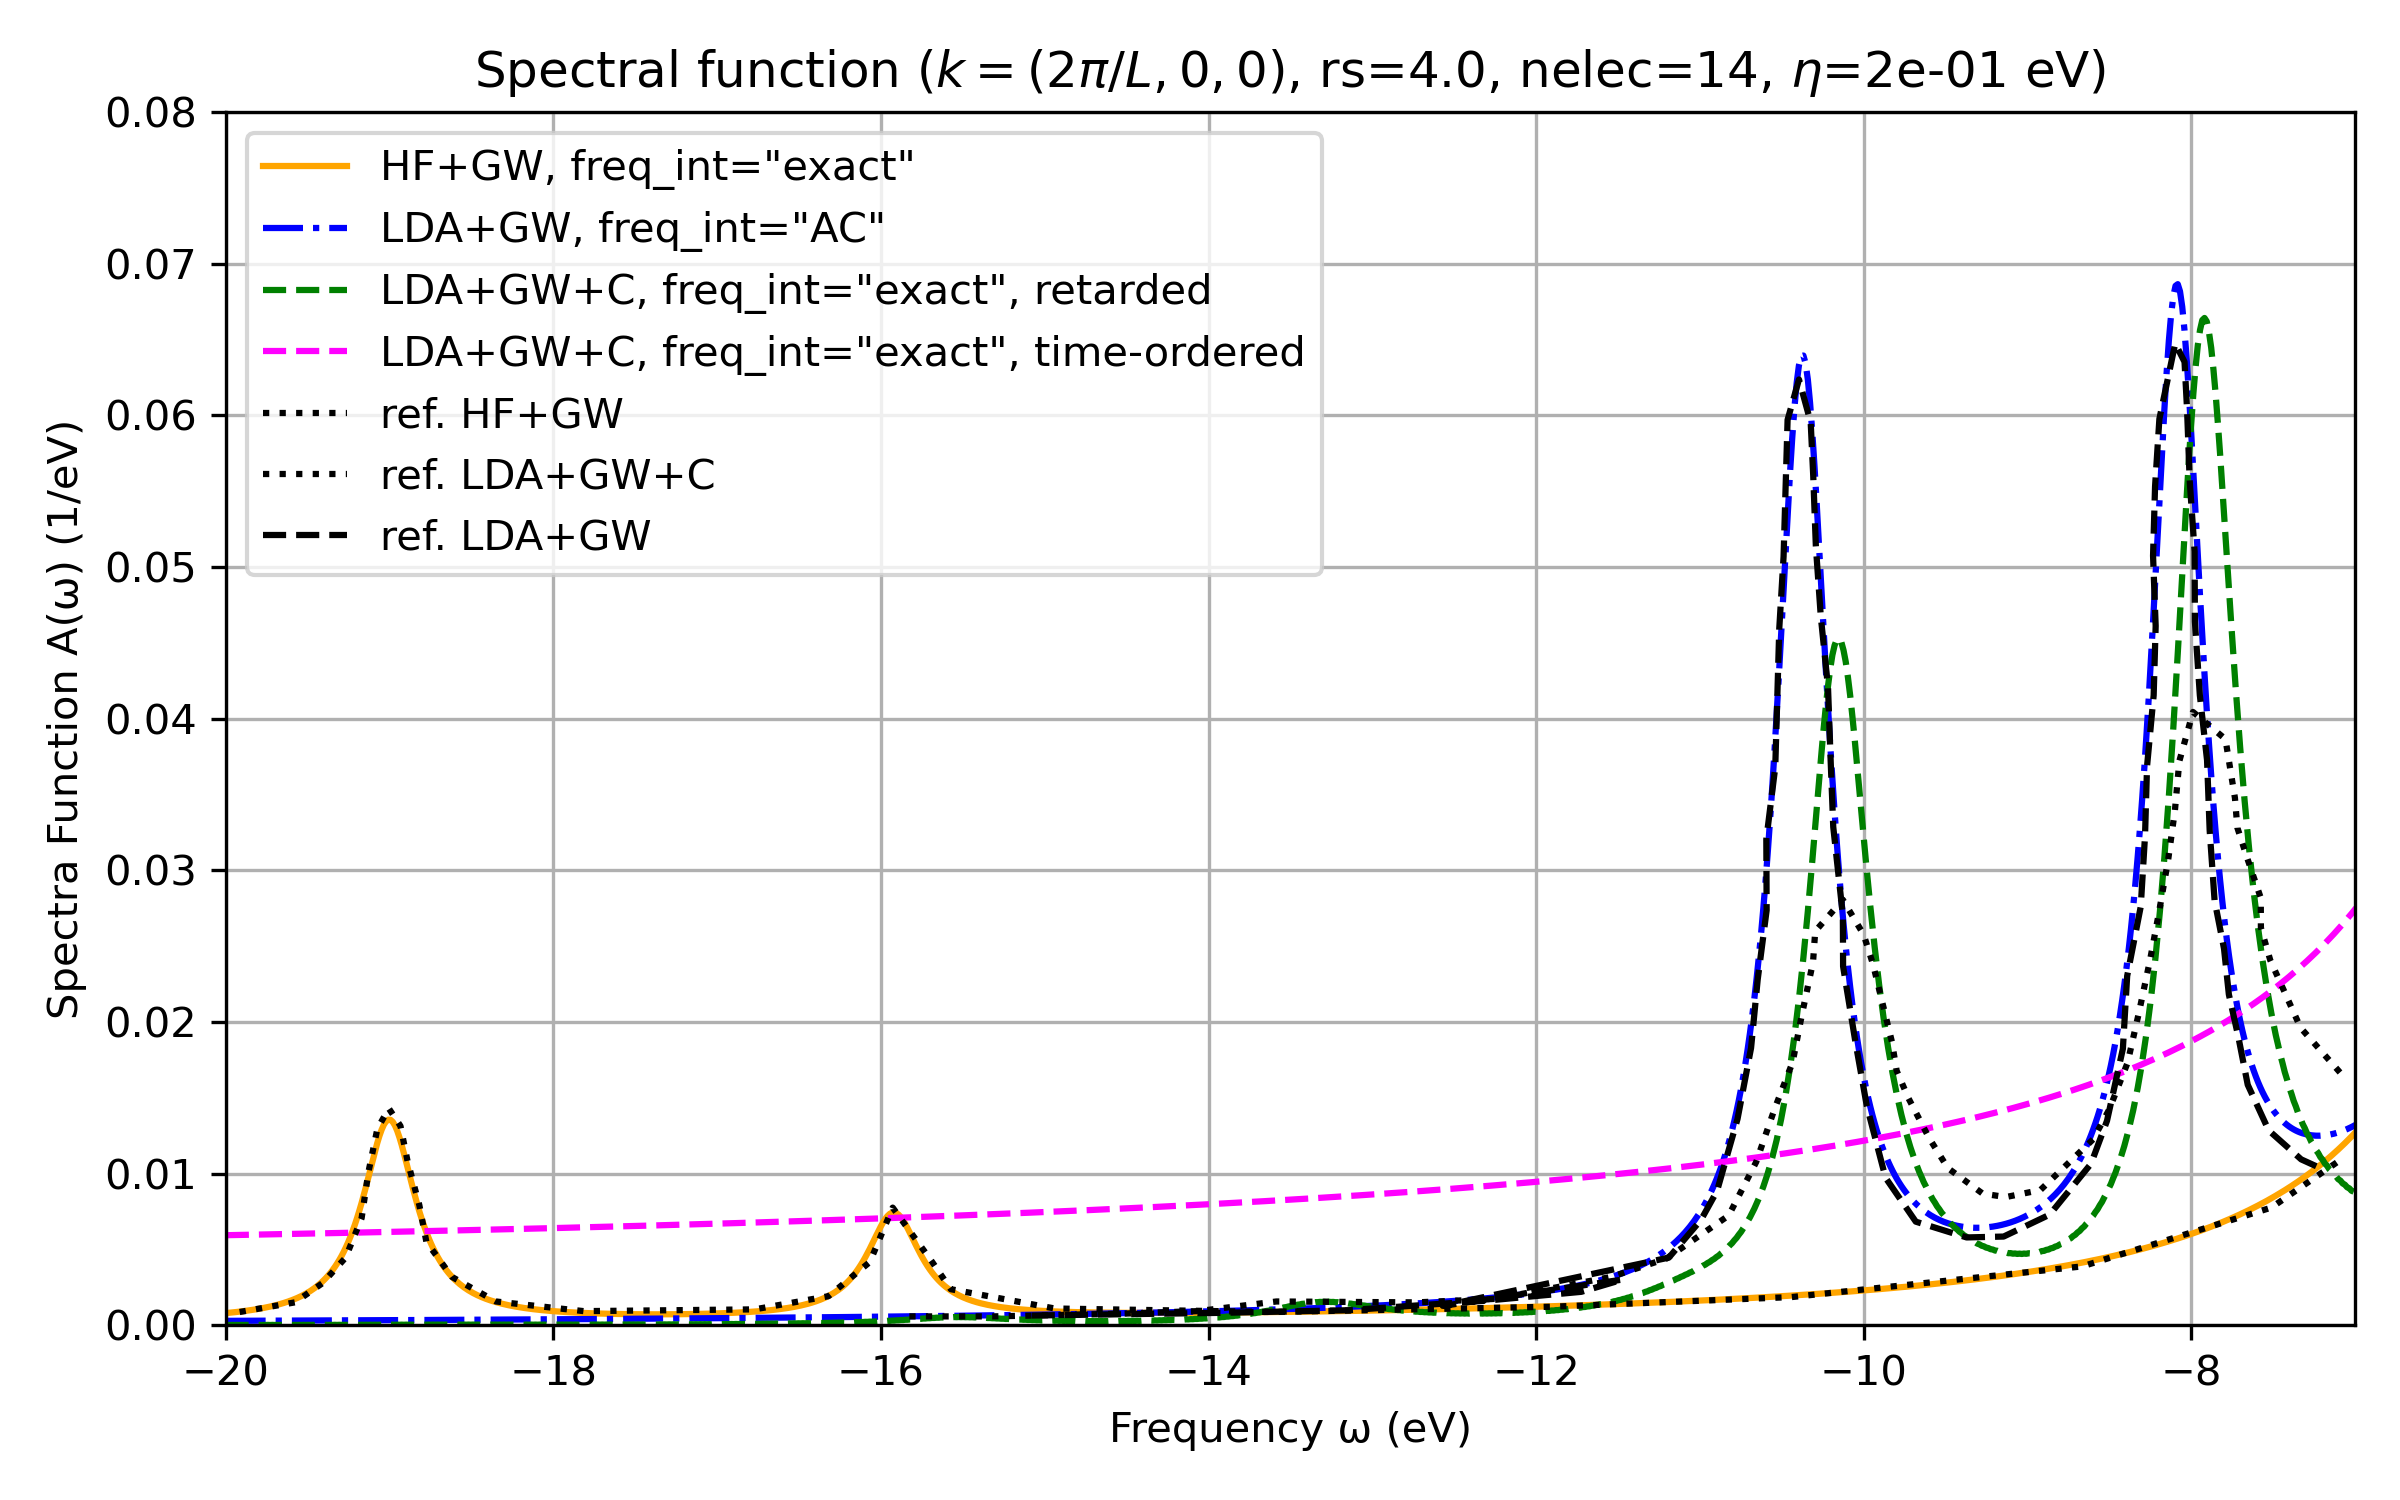
\includegraphics[width=\textwidth]{figs/v1_pidx6_rs4.0.png}
\end{figure}
\end{frame}
\begin{frame}
\frametitle{Time ordering}
\begin{align}
    A_{k}(\omega)
 & =\frac{1}{\pi}\left|\operatorname{Im} G_{k}^{\mathrm{T}}(\omega)\right|=-\frac{1}{\pi} \operatorname{Im} G_{k}^{\mathrm{R}}(\omega)
\end{align}
\pause
Retarded:
\begin{align}
    G^R_k(t)&= G^R_{0, k}(t) \exp \left[-i \Sigma_k^{\mathrm{x}} t+C^R_k(t)\right] \\
C^R_k(t) & =\pi^{-1} \int d \omega\left|\operatorname{Im} \Sigma^R_k\left(\omega+E_k^{G W}\right)\right|\left(e^{-i \omega t}+i \omega t-1\right) / \omega^2
\end{align}
\pause
vs. time ordered:
\begin{align}
    G_{k}^{\mathrm{T}}(t)&=\mathrm{i} \Theta(-t) e^{-\mathrm{i} \epsilon_k t} e^{C_{ k}^{\mathrm{T}}(t)} \\
C_{k}^{\mathrm{T}}(t) & =\int d \omega \frac{\beta_k^{ -}(\omega)}{\omega^2}\left(e^{-i \omega t}+i \omega t-1\right)\\
\beta_k^{ -}(\omega) & = \left|\operatorname{Im} \Sigma_k^R\left(\omega+\epsilon_k\right)\right| \theta\left[-\left(\epsilon_{k_F}-\epsilon_k-\omega\right)\right]
\end{align}
\end{frame}
\begin{frame}
\frametitle{Plasmon-pole model}
\begin{equation}
\Sigma^c(\mathbf{k}, \omega)=\sum_{\mathbf{q}} v(q) A(q)\left[\frac{1-f_{\mathbf{k}-\mathbf{q}}}{\omega-\varepsilon_{\mathbf{k}-\mathbf{q}}-\tilde{\omega}(q)+i \eta}+\frac{f_{\mathbf{k}-\mathbf{q}}}{\omega-\varepsilon_{\mathbf{k}-\mathbf{q}}+\tilde{\omega}(q)+i \eta}\right]
\end{equation}
\pause
with 
\begin{align}
A(q) &=-\frac{\pi}{2} \frac{\Omega(q)}{\tilde{\omega}(q)} \\
\Omega(q)^2
&= 4\pi n \\
\tilde{\omega}(q)^2 &= \frac{\Omega(q)^2}{1 - \epsilon^{-1}(q, \omega=0)} \\
\operatorname{Re} \epsilon^{-1}(q, \omega) &\approx 1+\frac{\Omega(q)^2}{\omega^2-\tilde{\omega}(q)^2}
\end{align}
\pause
Do we need finite-size corrections?
\end{frame}
\section{Future directions}
\begin{frame}
\frametitle{Future directions}
\begin{itemize}
    \item Verify that doing plasmon-pole model for the frequency integration reproduces the reference
    \pause
    \item Implement additional frequency integration schemes
\end{itemize}
\end{frame}